% !TEX root = main.tex

\section{恢复系统} % Chap 16
\subsection{故障分类}
\begin{itemize}
	\item 事务故障(failure)
	\begin{itemize}
		\item 逻辑错误:事务由于某些内部条件而无法继续正常执行,如非法输入。
		\item 系统错误:系统进入一种不良状态(如死锁),事务无法正常运行,但是之后某个时间点能够重新执行。
	\end{itemize}
	\item 系统崩溃(crash):硬件故障,或数据库软件/操作系统的漏洞,导致易失性存储器内容丢失,事务停止。
	\item 磁盘故障(failure):数据传送过程中由于磁头损坏或故障造成的磁盘块上内容丢失。
\end{itemize}

恢复算法包括两个部分:
\begin{itemize}
	\item 在正常事务执行过程中做的动作,获得之后能够从错误中恢复的信息
	\item 在数据库发生故障时执行的动作,使得恢复后可以确保原子性、一致性和持久性
\end{itemize}

\subsection{恢复与原子性}
记录以下操作(所有日志都应该在操作前被写入)
\begin{itemize}
\item 当一个事务$T_i$开始时,它会记录一个日志$<T_i\quad\text{start}>$。
\item 在每一个写操作$write(X)$之前,记录日志$<T_i,X,V_1,V_2>$,其中$V_1$是旧值,$V_2$是新值。
\item 当$T_i$完成它最后一条指令时,记录日志$<T_i\quad\text{commit}>$被写入。只有当提交日志被写入稳定存储,这个事务才能被称为已提交。
\end{itemize}

事务回滚操作:
\begin{enumerate}
	\item \textbf{从后往前}扫描日志,对于所发现的$T_i$的每个形如$<T_i,X_j,V_1,V_2>$的日志记录:
	\begin{enumerate}
		\item 值$V_1$被写到数据项$X_j$中,且
		\item 往日志中写一个特殊的只读日志记录$<T_i,X_j,V_1>$,其中$V_1$是在本次回滚中数据项$X_j$恢复成的值。这种日志称作补偿日志记录(compensation log record)。
	\end{enumerate}
	\item 一旦发现$<T_i,start>$的日志记录,就停止从后往前扫描,并往日志中写一个$<T_i,abort>$的日志记录
\end{enumerate}

使用日志来重做(redo)和撤销(undo)事务:
\begin{itemize}
	\item Redo指写入新值$V_2$
	\item Undo指写回旧值$V_1$
\end{itemize}

Redo阶段:
\begin{itemize}
	\item 找到最后一个检查点$<\text{checkpoint}\quad L>$,设置undo-list为$L$
	\item 从上面的检查点做前向扫描,
	\begin{itemize}
		\item 若$<T_i,X_j,V_1,V_2>$被发现,则重做,将$V_2$写到$X_j$
		\item 当$<T_i\quad\text{start}>$被发现,则添加$T_i$到undo-list中
		\item 当$<T_i\quad\text{commit}>$或$<T_i\quad\text{abort}>$被发现,从undo-list中移除$T_i$
	\end{itemize}
\end{itemize}

Undo阶段:从后面往前扫日志
\begin{itemize}
	\item 若$<T_i,X_j,V_1,V_2>$被发现且$T_i$在undo-list中,则
	\begin{itemize}
		\item 执行undo,将$V_1$写到$X_j$
		\item 写日志$<T_i,X_j,V_1>$
	\end{itemize}
	\item 当$<T_i\quad\text{start}>$被发现且$T_i$在undo-list中,则
	\begin{itemize}
		\item 写日志$<T_i\quad\text{abort}>$
		\item 将$T_i$从undo-list中移除
	\end{itemize}
	\item 当undo-list为空时停止,即$<T_i\quad\text{start}>$在undo-list中被每一个事务找到
\end{itemize}
\begin{figure}[H]
\centering
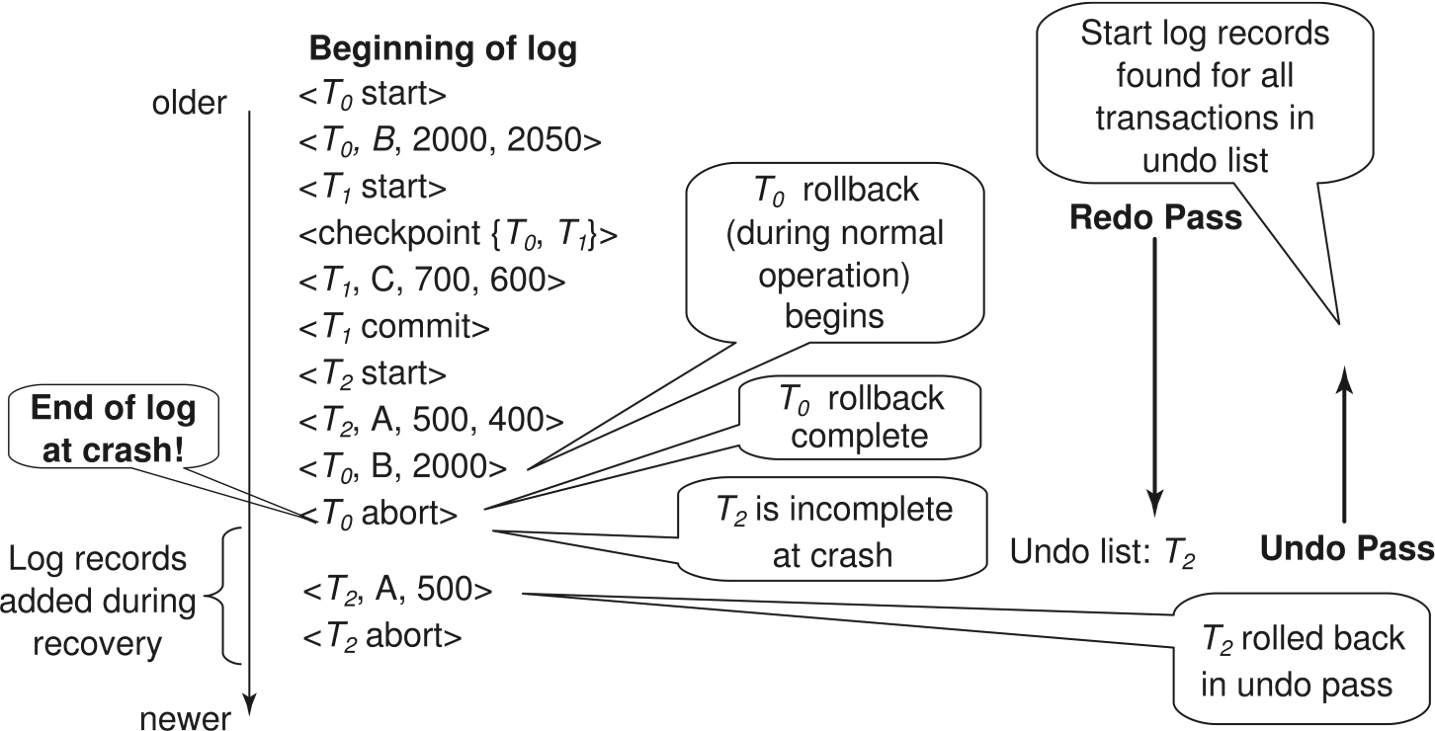
\includegraphics[width=0.8\linewidth]{fig/recovery.png}
\end{figure}

但每个操作都要写日志就很慢,因此采用检查点(checkpoint)进行打包。
\begin{figure}[H]
\centering
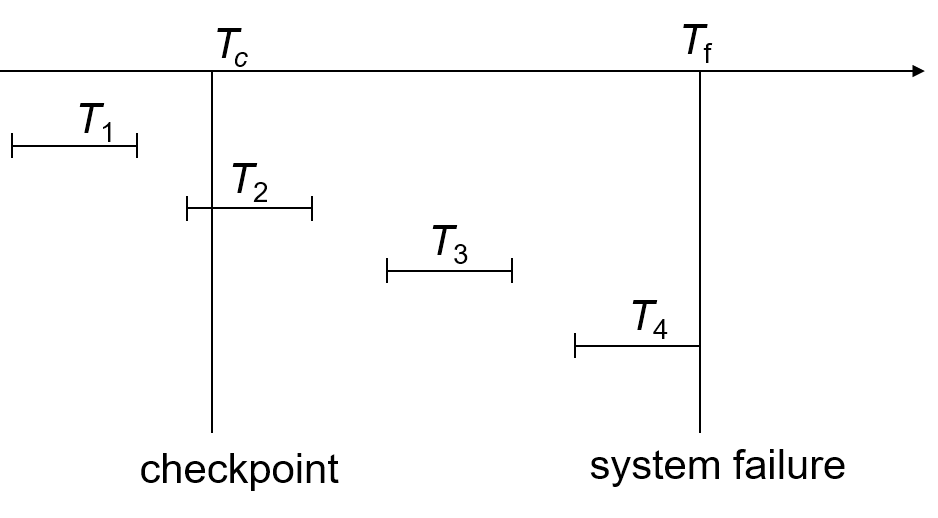
\includegraphics[width=0.6\linewidth]{fig/checkpoints_eg.png}
\end{figure}
其中,
\begin{itemize}
	\item $T_1$可被忽略,因为已经写入磁盘
	\item 检查点是$T_c$,故$T_2$和$T_3$需要Redo
	\item 而$T_4$需要undo
\end{itemize}